\newcommand*{\SHORTPRES}{}%
\documentclass[serif,mathserif]{beamer}
\usepackage{amsmath, amsfonts, epsfig, xspace}
\usepackage{algorithm,algorithmic}
\usepackage{pstricks,pst-node}
\usepackage{moreverb}
\usepackage[normal,tight,center]{subfigure}
\setlength{\subfigcapskip}{-.5em}
\usepackage{beamerthemesplit}
\usetheme{lankton-keynote}

\author{S\'ebastien Bourdeauducq}

\title{Migen}
\subtitle{A Python toolbox for building complex digital hardware}

\date{2012}

\begin{document}

\maketitle

\begin{frame}
\begin{centering}

\includegraphics[width=5cm]{migen_logo.png} \\

\includegraphics[width=\textwidth]{migenblock.png}
\end{centering}
\end{frame}

\begin{frame}[fragile]
\frametitle{FHDL}
\begin{itemize}
\item Python as a meta-language for HDL
\begin{itemize}
\item Think of a \verb!generate! statement on steroids
\end{itemize}
\item Restricted to synchronous circuits
\item Designs are split into:
\begin{itemize}
\item synchronous statements $\Longleftrightarrow$ \verb!always @(posedge clk)! \\
(VHDL: \verb!process(clk) begin if rising_edge(clk) then!)
\item combinatorial statements $\Longleftrightarrow$ \verb!always @(*)! \\
(VHDL: \verb!process(all inputs) begin!)
\end{itemize}
\item Statements expressed using nested Python objects
\begin{itemize}
\item Various syntax tricks to make them look nicer \\
\textit{("internal domain-specific language")}
\end{itemize}
\end{itemize}
\end{frame}

\begin{frame}[fragile]
\frametitle{FHDL crash course}
\begin{itemize}
\item Basic element is \verb!Signal!.
\begin{itemize}
\item Similar to Verilog \verb!wire/reg! and VHDL \verb!signal!.
\end{itemize}
\item Signals can be combined to form expressions.
\begin{itemize}
\item e.g. \verb!(a & b) | c!
\end{itemize}
\item Signals have a \verb!eq! method that returns an assignment to that signal.
\begin{itemize}
\item e.g. \verb!x.eq((a & b) | c)!
\end{itemize}
\item Assignments are collected into lists.
\begin{itemize}
\item Control structures (\verb!If!, \verb!Case!) also supported.
\end{itemize}
\item List of combinatorial assignments + list of synchronous assignments + ``goodies'' = \verb!Fragment!
\item Fragments can be combined to form a design to be converted for synthesis or simulated.
\end{itemize}
\end{frame}

\begin{frame}[fragile]
\frametitle{Conversion for synthesis}
\begin{itemize}
\item FHDL is entirely convertible to synthesizable Verilog 
\item VHDL proposed, in development\footnote{https://github.com/peteut/migen}
\end{itemize}
\begin{verbatimtab}
>>> from migen.fhdl.structure import *
>>> from migen.fhdl import verilog
>>> counter = Signal(16)
>>> o = Signal()
>>> comb = [o.eq(counter == 0)]
>>> sync = [counter.eq(counter + 1)]
>>> f = Fragment(comb, sync)
>>> print(verilog.convert(f, ios={o}))
\end{verbatimtab}
\end{frame}

\begin{frame}[fragile]
\begin{verbatimtab}
module top(input sys_rst, input sys_clk, output o);

reg [15:0] counter;

assign o = (counter == 1'd0);

always @(posedge sys_clk) begin
        if (sys_rst) begin
                counter <= 1'd0;
        end else begin
                counter <= (counter + 1'd1);
        end
end

endmodule
\end{verbatimtab}
\end{frame}

\begin{frame}[fragile]
\frametitle{Simulation}
\begin{itemize}
\item Fragments contain a list of Python functions to execute at each clock cycle during simulations.
\item Simulator provide read and write methods that manipulate FHDL \verb!Signal! objects.
\item Powerful Python features, e.g. generators:
\end{itemize}
\begin{verbatimtab}
def my_generator():
        for x in range(10):
                t = TWrite(x, 2*x)
                yield t
                print("Wrote in " + str(t.latency) + " cycle(s)")
                # Insert some dead cycles to simulate bus inactivity.
                for delay in range(prng.randrange(0, 3)):
                        yield None
master1 = wishbone.Initiator(my_generator())
master2 = asmibus.Initiator(my_generator(), port)
\end{verbatimtab}
\end{frame}

\begin{frame}[fragile]
\frametitle{Pytholite}
\begin{itemize}
\item Some of those generators are even synthesizable :)
\item Output: FSM + datapath
\item Lot of room for improvement (mapping, scheduling, recognized subset)
\item One application today: high-speed control of the analog RF chain of a radar
\end{itemize}
\begin{verbatimtab}
def generator():
        for i in range(10):
                yield TWrite(i, 0)
bus_if = wishbone.Interface()
pl = make_pytholite(generator,
        buses={"def": bus_if})
f = pl.get_fragment()
\end{verbatimtab}
\end{frame}

\begin{frame}[fragile]
\frametitle{Verilog/VHDL interface}
\begin{itemize}
\item Fragments can contain instances of external Verilog or VHDL modules.
\item In development: Migen ``embedded'' mode\footnote{https://github.com/Florent-Kermarrec/migen}
\begin{itemize}
\item Similar to PHP's \verb!<?! and \verb!?>!
\item Write most of your code in Verilog/VHDL, insert Python code between \verb![-! and \verb!-]!
\end{itemize}
\end{itemize}
\end{frame}

\begin{frame}[fragile]
\frametitle{Bus support}
\begin{itemize}
\item Wishbone\footnote{http://www.opencores.org}
\item SRAM-like CSR
\item DFI \footnote{http://www.ddr-phy.org}
\item ASMI
\end{itemize}
\centering 
\includegraphics[height=1cm]{opencores.png} 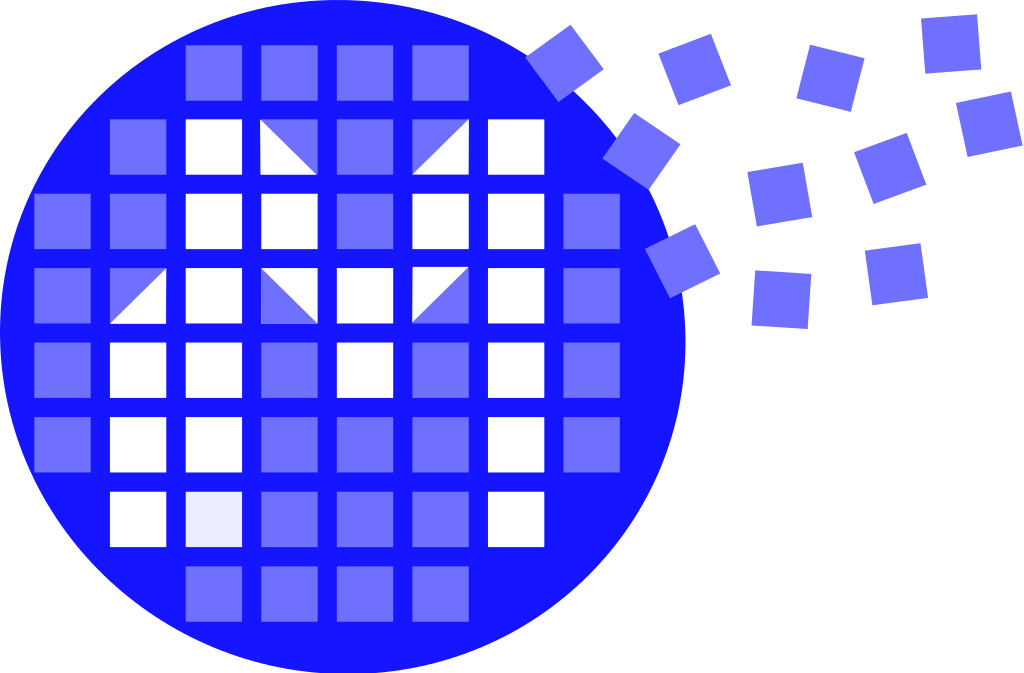
\includegraphics[height=1cm]{milkymist.png} 
\includegraphics[height=1cm]{dfi.png}
\begin{verbatimtab}
wishbonecon0 = wishbone.InterconnectShared(
        [cpu0.ibus, cpu0.dbus],
        [(lambda a: a[26:29] == 0, norflash0.bus),
         (lambda a: a[26:29] == 1, sram0.bus),
         (lambda a: a[26:29] == 3, minimac0.membus),
         (lambda a: a[27:29] == 2, wishbone2asmi0.wishbone),
         (lambda a: a[27:29] == 3, wishbone2csr0.wishbone)])
\end{verbatimtab}
\end{frame}

\begin{frame}[fragile]
\frametitle{CSR banks and interrupt controllers}
\begin{verbatimtab}
_rxtx = RegisterRaw("rxtx", 8)
_divisor = RegisterField("divisor", 16, reset=int(clk_freq/baud/16))
_tx_event = EventSourceLevel()
_rx_event = EventSourcePulse()
events = EventManager(_tx_event, _rx_event)
bank = csrgen.Bank([_rxtx, _divisor] + events.get_registers(),
     address=address)
\end{verbatimtab}
\end{frame}

\ifdefined\SHORTPRES
\begin{frame}
\frametitle{ASMI}
ASMI (Advanced System Memory Infrastructure) key ideas
\begin{itemize}
\item Speed is beautiful: optimize for maximum performance
\item Only introduce bottlenecks that DRAM already has
\item Wide transaction issue with dedicated slots
\item Operate several FSMs concurrently to manage each bank
\item In a frequency-ratio system, issue multiple DRAM commands from different bank FSMs in a single cycle
\begin{itemize}
\item PHY uses SERDES to handle I/O
\item FPGAs are horribly and painfully SLOW, so we need such tricks even for DDR333 (2002!!!)
\item and still we can only reach 1.8Gbps/pin on a Virtex-7, while commodity GPUs have 5Gbps/pin
\end{itemize}
\item Reorder commands to minimize dead times (row switches, read-write turnaround)
\end{itemize}
\end{frame}
\else
\begin{frame}
\frametitle{ASMI}

\includegraphics[width=\textwidth]{asmi_topology.png} \\
ASMI (Advanced System Memory Infrastructure) topology
\end{frame}

\begin{frame}
\frametitle{For master devices}
\begin{itemize}
\item Each master has one or several dedicated request slots
\item At any slot, master presents valid address and WE and asserts request
\item Slot number (\textit{tag}) appears on shared bus
\begin{itemize}
\item nb: this sharing is not a performance bottleneck, DRAM data pins already have exact same sharing
\end{itemize}
\item For a read: followed by data from DRAM in the next cycle
\item For a write: master is required to output valid data in the next cycle
\end{itemize}
\end{frame}

\begin{frame}
\frametitle{Proposed memory controller}
Memory controller operates several \textit{bank machines} in parallel
\begin{itemize}
\item Each bank machine sees all outstanding requests for the DRAM bank it manages
\item Tracks open row, detects page hits
\item May reorder requests to optimize page hit rate
\item Ensures per-bank timing specifications are met (tRP, tRCD, tWR)
\item Generates DRAM-level requests (PRECHARGE, ACTIVATE, READ, WRITE)
\end{itemize}
\end{frame}

\begin{frame}
\frametitle{Proposed memory controller}
\textit{Command steering} stage picks final requests
\begin{itemize}
\item In a frequency-ratio system, may issue multiple commands from several bank machines in a single cycle
\begin{itemize}
\item PHY uses SERDES to handle I/O
\item FPGAs are horribly and painfully SLOW, so we need such tricks even for DDR333 (2002!!!)
\end{itemize}
\item May group writes and reads to reduce turnaround times
\item Ensures no read-to-write conflict occurs on the shared bidirectional data bus
\item Ensures write-to-read (tWTR) specification is met
\end{itemize}
\end{frame}
\fi

\begin{frame}
\frametitle{Migen support}
\begin{itemize}
\item Migen provides generic components only
\item e.g. memory controller and PHY are not included
\begin{itemize}
\item part of milkymist-ng\footnote{https://github.com/milkymist/milkymist-ng}
\item reference design available for Milkymist One board (DDR333 + Spartan-6)
\end{itemize}
\item Provides containers, bus simulation components, hub to manage requests, reorder buffer
\end{itemize}
\end{frame}

\begin{frame}
\frametitle{Dataflow programming}
\begin{itemize}
\item Representation of algorithms as a graph (network) of functional units
\item Similar to LabVIEW or Pure Data
\item Parallelizable and relatively intuitive
\item Migen provides infrastructure for actors (functional units) written in FHDL
\item Migen provides an actor library for DMA (Wishbone and ASMI), simulation, etc.
\end{itemize}
\end{frame}

\begin{frame}
\frametitle{Dataflow programming}
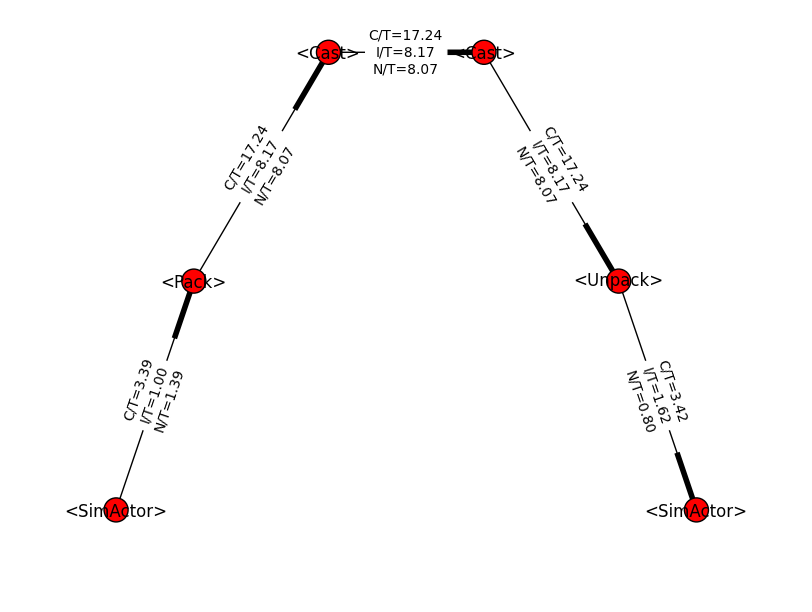
\includegraphics[width=\textwidth]{agperf.png}
\end{frame}

\begin{frame}
Migen is open source!
\begin{itemize}
\item GPLv3 with instantiation permissions
\item http://milkymist.org/3/migen.html
\item http://github.com/milkymist/migen
\item mailing list: http://lists.milkymist.org
\item IRC: Freenode \#milkymist
\end{itemize}

\centering 
\includegraphics[width=5cm]{migen_logo.png}

\end{frame}

\end{document}
